\documentclass{report}
\usepackage[a4paper, margin=0.5in]{geometry}
\usepackage{parskip}
\usepackage{graphicx}
\usepackage{caption}
\usepackage{amssymb}
\usepackage{amsmath}
\usepackage{algpseudocode}
\usepackage{algorithm}

\captionsetup[figure]{
  font = it,
  labelfont = bf
}

\begin{document}
  \begin{minipage}[b]{0.48\textwidth}
    \section*{Load balancing in standard kMeans}
    Suppose that the standard kMeans algorithm is executed in parallel by splitting between T threads the total points N. In this case the work load is easly divided equally between the threads. In fact we can calculate the total number of points to assign each thread by N/T; if N is not a multiple of T we will also have a reminder (r)
    \begin{equation}
      r = N \text{ mod } T < T
    \end{equation}
    If this is the case, we can simply assign the first r threads one more point, therefore in the end there will be r threads with N/T + 1 points and T - r threads with N/T points.

    \section*{Load balancing in Hamerly's algorithm}
    With Hamerly's algorithm, efficient load balancing is not as easy as in the standard version because, for every cycle, it is not neccessary to compute the distances for every points but only for critical ones. Because of this, if the points were simply divided among the threads, it might happen that some have many points while others could have few calculations to do.

    \begin{center}
      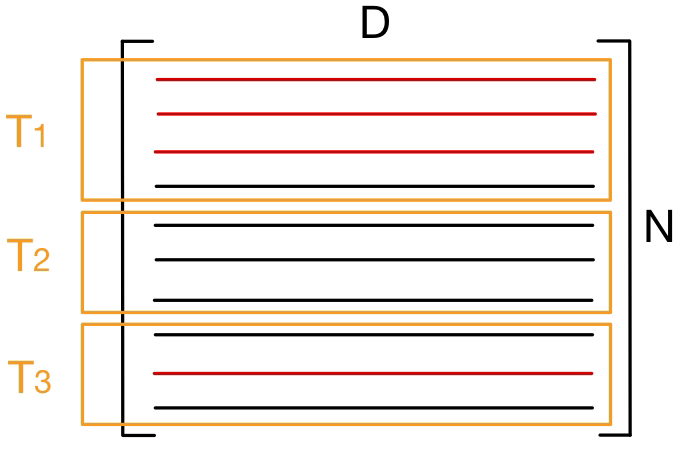
\includegraphics[width = 0.8\textwidth]{imgs/non_balances_hamerly.png}
      \captionof{figure}{Non balanced point division}
      \label{fig:non_bal_ham}
    \end{center}

    The Figure \ref{fig:non_bal_ham} shows an input matrix (N x D, where D is the data dimensionality) where critical points are not  equally distribuited. In this case, the first thread will have three critical points whereas the second thread will have zero.

    To implement an efficient load balacing, a more advanced strategy is needed and one possible solution will be presented in the following part of this report. 
    
    \subsection*{Points assigment for Hamerly's algorithm}
    First of all remember that, in the Hamerly's algorithm, after that each centroid moved it is neccessary to update the upper bound (ub) and the lower bound ($lu$) of each point. This operation can be done in parallel, since the update is indipendent between the points, and no special cautions are required when splitting the points because the work that has to be done is equal for each point. 

    During this phase, each thread will have a linked list where it adds every critical point that it finds, moreover every time it finds a critical it increments by one the value of a global array which has a length of T so that each thread has its own index to access.

    After that all points have been iterated a synchronization is required. During this sequential part it is calculated the total number of critical points that have been found, also, during this step, a second array is created that length
  \end{minipage}
  \hspace{0.15in}
  \raisebox{0in}{
  \begin{minipage}[b]{0.48\textwidth}
    At this point, every thread can insert, inside this new array, its critical points. In order to do that, every thread has to start inserting its values from the index which is equal to the sum of the number of criticals found by the previous threads.

    For example, if there are 3 threads and they found respectively [2, 3, 1] criticals then, they start inserting values from the 0, 2 and 5 (2 + 3) index. The objective of this step is to create an array containing all the critical points together because in this way it is possible to equally divide those critical between the threads. 

    If the total number of critical points is $N_c$ then, the number of criticals to assign each thread can be calculated as $N_c / T$. If $N_c$ is not a multiple of T, there will also be a remainder which can be handled the same way as in the standard case. Below is the pseudo code where N is the total numer of points and P is the array containing all points.

    \begin{algorithm}[H]
      \caption{kMeans class assigment pseudo-code}\label{alg:cap}
      \begin{algorithmic}
        \State --------------------------------------------- \Comment Sequentially
        \State Let $C_{max}$ be the centroid which moved the most 
        \State Let $C_{2nd}$ be the 2nd centroid which moved the most
        \State Let nC be the array with the number of criticals found by each thread 
        \State (Remainder) r = N \% T
        \State --------------------------------------------- \Comment In Parallel
        \State Let i be the id of the current thread 
        \State Let $L_i$ be the list of criticals found by the i-th thread

        \State$N_i = Int(N/T)$
        \State offset = r

        \If{$i < r$}
          \State $N_i = N_i + 1$
          \State offset = 0
        \EndIf

        \State
        \For{$j < N_i$}
          \State point = P[$i\cdot N_i + $ offset]
          \State point.ub = point.ub+ point.centroid.distance
          \If{point.centroid == $C_{max}$}
            \State point.lb = point.lb - $C_{2nd}.distance$
          \Else
            \State point.lb = point.lb - $C_{max}.distance$
          \EndIf

          \If{point.$ub>$ point.lb}
            \State $L_i$.push(point)
            \State nC[i] = nC[i] + 1
          \EndIf
        \EndFor
        \State --------------------------------------------- \Comment Sequentially 
        \State sum = 0
        \For{j $<$ nC.length}
          \State sum = sum + nC[j]
        \EndFor

        \State Let A be the array of all the criticals (A.length = sum)
        \State --------------------------------------------- \Comment In Parallel 
        \State index = 0
        \For{j $<$ i}
          \State index = index + nC[j]
        \EndFor
        \State 
        \For{j $<$ nC[i]}
          \State A[index + j] = $L_i$.pop 
        \EndFor
      \end{algorithmic}
  \end{algorithm}
  \end{minipage}}

  \newpage

  \begin{minipage}[b]{0.48\textwidth}
    \subsection*{Insight into the opseudo code}
    Because some of the steps in the pseudocode may not be immediate in understanding what they do and why they are used, this part will give an overview of those instructions that may be less clear.

    \begin{algorithm}[H]
      \caption{The offset variable}
      \begin{algorithmic}
        \State offset = r

        \If{$i < r$}
          \State offset = 0
        \EndIf
      \end{algorithmic}
    \end{algorithm}

    The need of this variable comes from the fact that the first r threads (where r is the remainder of N/T) have to access N/T + 1 elements while the other threads have to access N/T this inequality is the reason why we need to introduce the variable offset.

    Suppose we have N = 20 and k = 3 (where k is the number of threads) then
    \begin{equation*}
      N_i = Int(20 / 3) = 6 \text{ and } r = 20 \text{ mod } 3 = 2
    \end{equation*}
    Therefore the first two thread have to access 7 elements while the last one will acces 6. Which from the indeces point of view would mean that the
    \begin{equation*}
      \text{Thread1 indices} \rightarrow [0, 6]
    \end{equation*}
    \begin{equation*}
      \text{Thread2 indices} \rightarrow [7, 13]
    \end{equation*}
    \begin{equation*}
      \text{Thread3 indices} \rightarrow [14, 19]
    \end{equation*}

    To calculate the first two set of indeces it is easy because we can just use the thread id (i) and the following formula
    \begin{equation}\label{eq:ind1set}
      \mathbf{[}(i - 1) \cdot (N_i + 1) \hspace{0.05in}\mathbf{,}\hspace{0.05in} (i - 1) \cdot (N_i + 1) + N_i\mathbf{]}
    \end{equation}

    The problem comes for the other threads, in this case the third one. For all the thread that access $N_i$ values (not $N_i + 1$) another equation has to be used
    \begin{equation*}
      \mathbf{[}(i - 1) \cdot N_i + r \hspace{0.05in}\mathbf{,}\hspace{0.05in} (i - 1) \cdot N_i + r + N_i - 1\mathbf{]}
    \end{equation*}

    The reason why we need to change equation to calculate the second groups of indeces is because every time we use the equation (\ref{eq:ind1set}) we introduce a shift of one with respect to the indeces that would have been calculated as
    \begin{equation*}
      \mathbf{[}(i - 1) \cdot N_i \hspace{0.05in}\mathbf{,}\hspace{0.05in} (i - 1) \cdot N_i + N_i - 1\mathbf{]}
    \end{equation*}
    Which would be the equation to use if all thread were to access $N_i$ points.

    Since we use equation (\ref{eq:ind1set}) r times the shift will be r in the end. 
    Finally, notice the if statement because when applying equation (\ref{eq:ind1set}) the offset is not needed therefore we need to distiguish between the two cases.

    Note also that in all equations, (i - 1) was used because we considered thread ids starting from 1, but it is just a convention, if the indexes started from 0 then it would have been correct to use only i.

    \begin{algorithm}[H]
      \caption{$N_i$ increment}
      \begin{algorithmic}
        \If{$i < r$}
          \State $N_i = N_i + 1$
        \EndIf
      \end{algorithmic}
    \end{algorithm}
  \end{minipage}
  \hspace{0.1in}
  \raisebox{2.5in}{
  \begin{minipage}[b]{0.48\textwidth}
    This if statement is implemented to increase by one the number of points that the first r threads have to access.

    \begin{algorithm}[H]
      \caption{point.centroid.distance}
      \begin{algorithmic}
        \State point.ub = point.ub+ point.centroid.distance
      \end{algorithmic}
    \end{algorithm}

    Through point.centroid we access the centroid assigned to the point and with centroid.distance we access the distance taken by the centroid during its last movement.

    At every iteration the upper bound of each point, which is accessed by point.ub, has to be updated and the new value will be: point.ub = point.ub + point.centroid.distance. 

    \begin{algorithm}[H]
      \caption{lower bound update}
      \begin{algorithmic}
        \If{point.centroid == $C_{max}$}
          \State point.lb = point.lb - $C_{2nd}.distance$
        \Else
          \State point.lb = point.lb - $C_{max}.distance$
        \EndIf
      \end{algorithmic}
    \end{algorithm}

    When it comes to updating the lower limit, the first thing to check is whether the centroid that moved the most is also the one assigned to the point. In this case, the lower limit cannot be updated with the distance of that centroid because it has already been used for the upper limit, but in this case the distance taken from the second centroid that moved the most has to be used.

    \begin{algorithm}[H]
      \caption{lower bound update}
      \begin{algorithmic}
        \State index = 0
        \For{j $<$ i}
          \State index = index + nC[j]
        \EndFor
      \end{algorithmic}
    \end{algorithm}

    This is the part where each thread calculate the index from where it has to start inserting the vales in the global array containing all the critical points (i is always the id of the current thread).

    \begin{algorithm}[H]
      \caption{add values to the global array}
      \begin{algorithmic}
        \For{j $<$ nC[i]}
          \State A[index + j] = $L_i$.pop 
        \EndFor       
      \end{algorithmic}
    \end{algorithm}
    This is the last part of the algorithm where every thread inserts into the global array the value of its list.
  \end{minipage}}
\end{document}